\section{Testing Outside \sedflow~Training Range} \label{sec:fail}
For a small number of NSA galaxies, 588 out of 33,884, \sedflow~does not
produce valid posteriors. 
The normalizing flow of \sedflow~generates posteriors that are entirely outside
of the prior volume because the photometry or uncertainties of the NSA galaxies
lie outside of the support of the \sedflow~training data
(Section~\ref{sec:training}). 
These galaxies lie outside of the support for two reasons: 
(1) they have unusually high photometric uncertainties that are not accounted
for in our noise model or 
(2) they have photometric colors that cannot be modeled by our SED model. 
In Figure~\ref{fig:fail}, we present the distribution of photometric
magnitudes, uncertainties, and redshift ($\bfi{x} = \{f_X, \sigma_X, z\}$) of
these NSA galaxies. 
We mark galaxies that are outside the \sedflow~training data support (black)
due to (1) in orange and (2) in blue. 

\begin{figure}
\begin{center}
    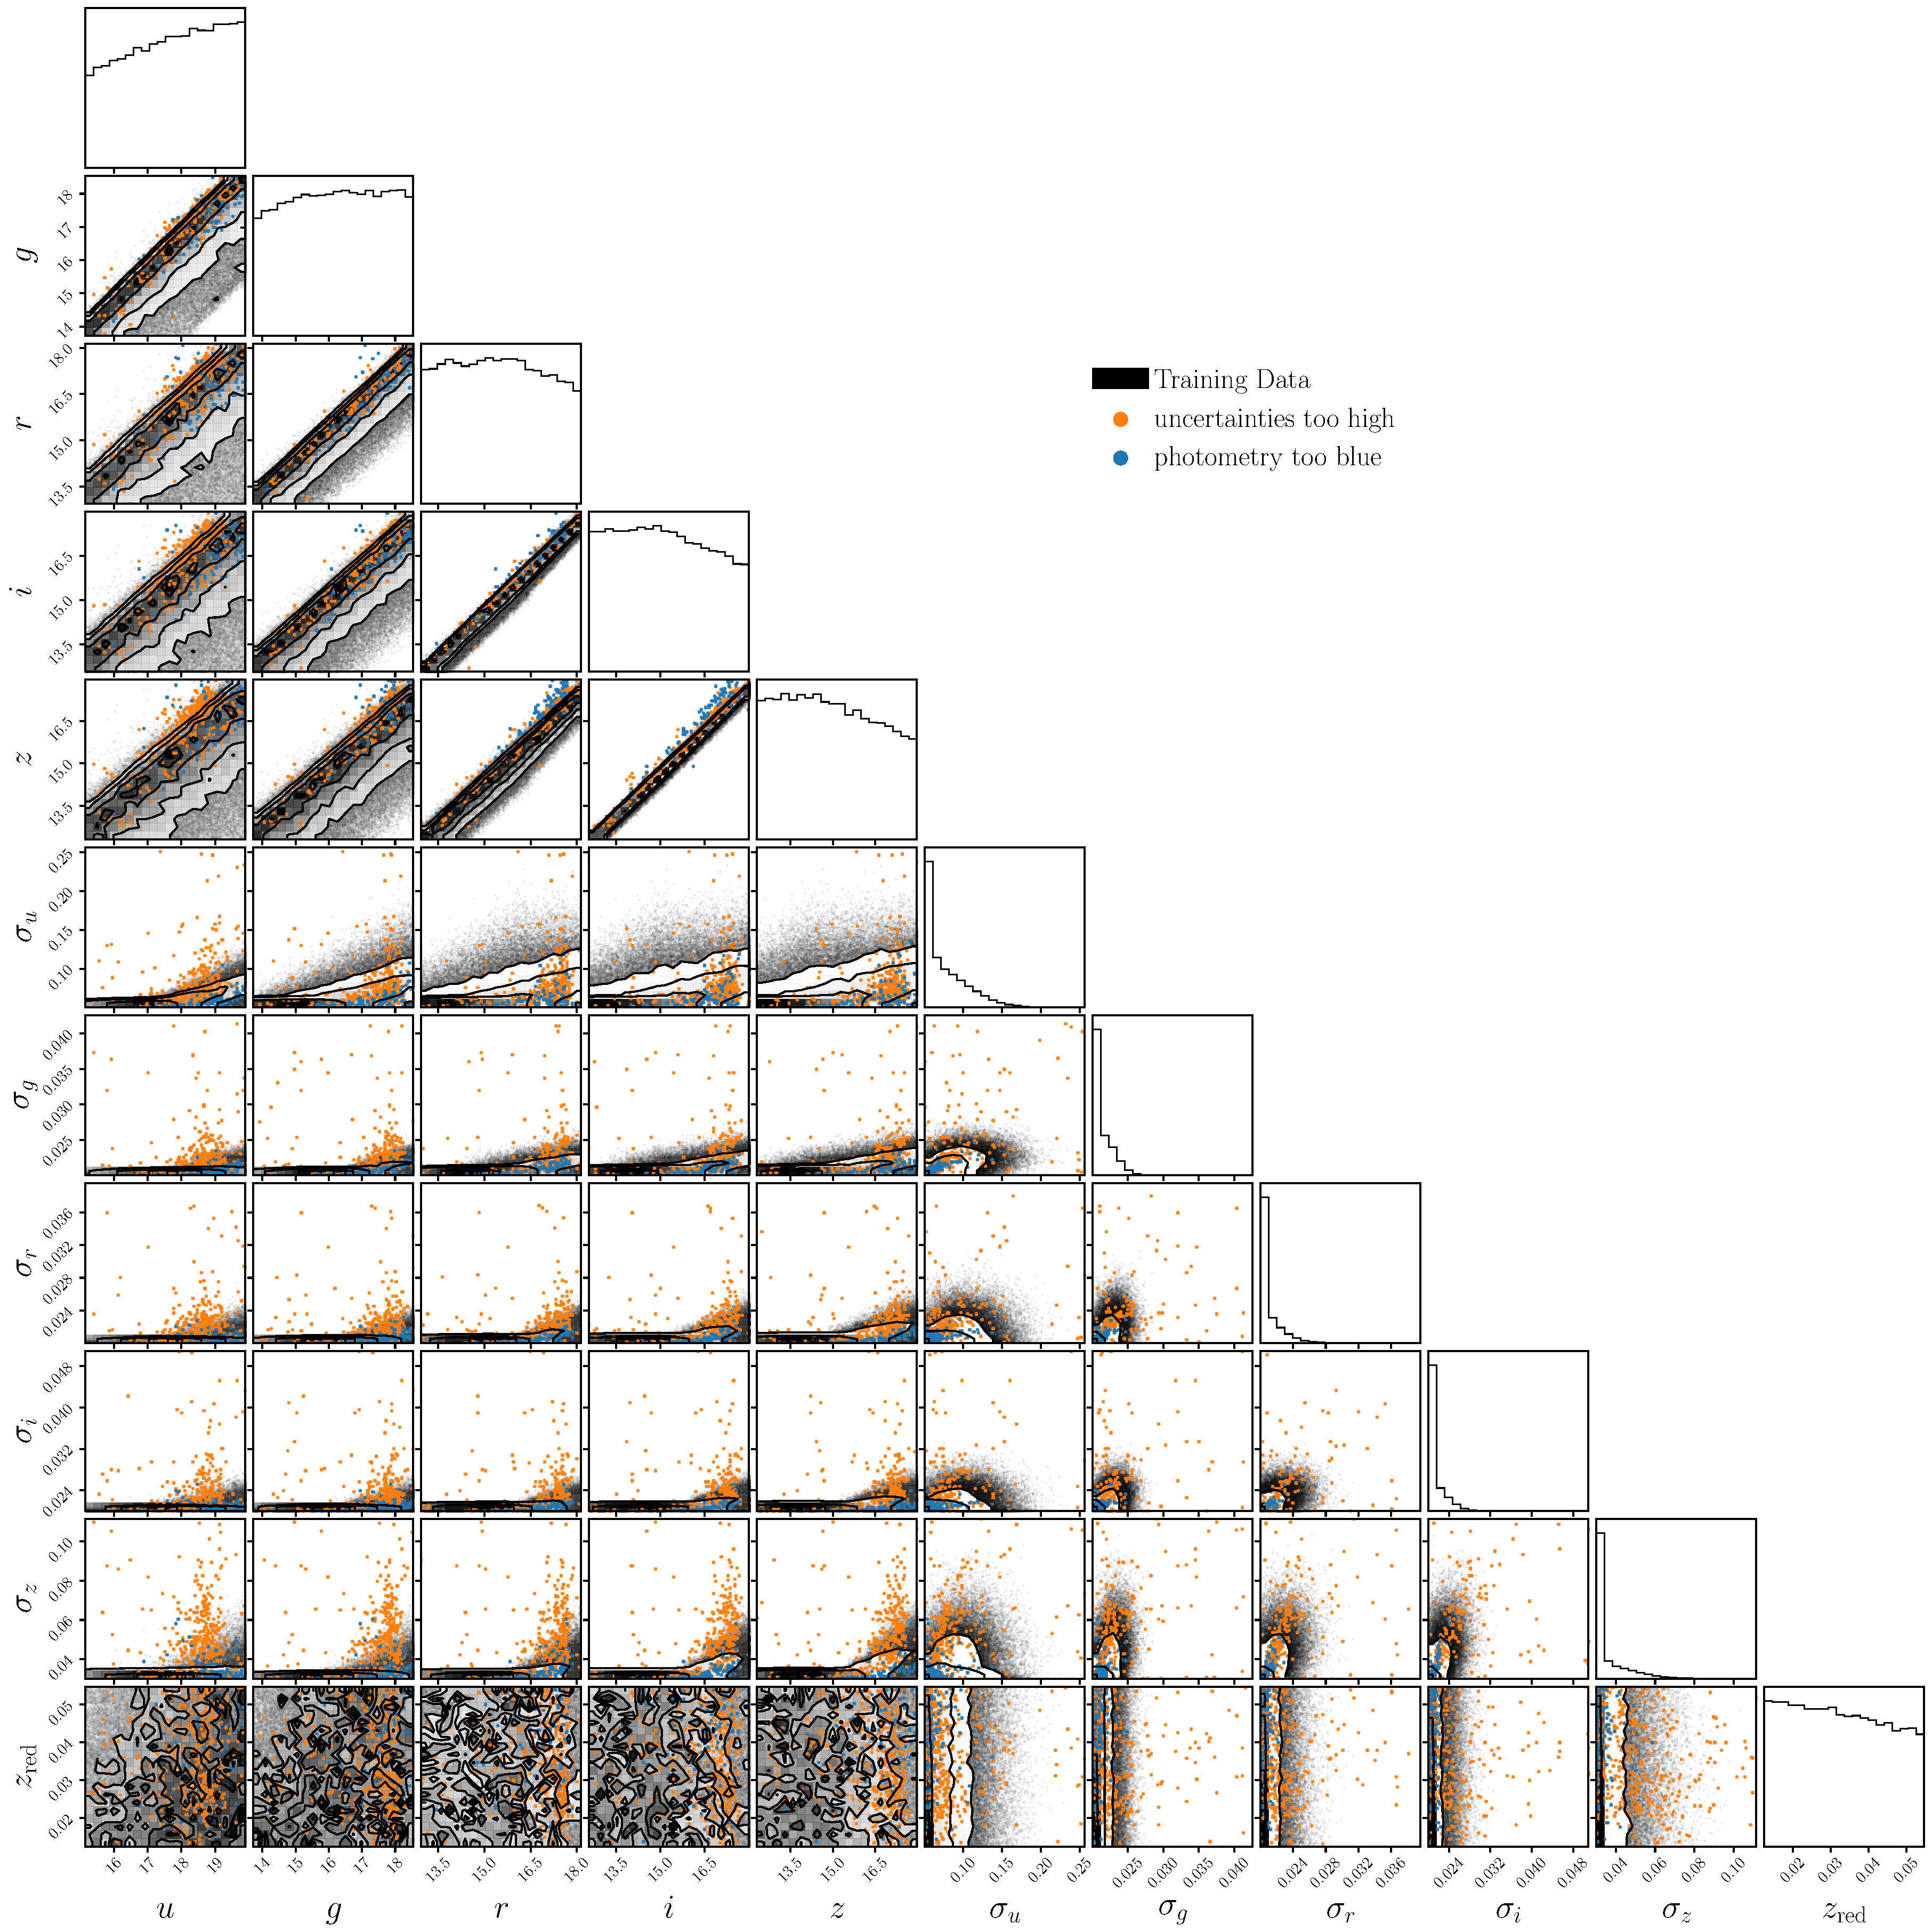
\includegraphics[width=0.9\textwidth]{figs/fails.pdf}
    \caption{\label{fig:fail}
    The distribution of photometric magnitudes, uncertainities, and redshift of
    NSA galaxies for which \sedflow~does not produce valid posteriors (blue or
    orange). 
    These galaxies lie outside of the suport of the \sedflow~training data
    (black) so \sedflow~cannot accurately estimate their posteriors. 
    We mark the NSA galaxies that have unusually high photometric uncertainties
    that are not accounted for in our noise model in orange and galaxies that
    have photometric colors that cannot be modeled by our SED model in blue. 
    }
\end{center}
\end{figure}
% paragraph discussing photometric uncertainty outliers
We classify NSA galaxies as (1) in Figure~\ref{fig:fail}, if they have
$\sigma_X$ that is unusually high for a given $f_X$ in at least one photometric
band: $\sigma_X > \mu_{\sigma_X}(f_X) + 3 \sigma_{\sigma_X}(f_X)$
(see Eq.~\ref{eq:noise}). 
There are 490 NSA galaxies without valid \sedflow~posteriors due to (1).
Many of these galaxies lie well beyond the locus of training data points. 
The \sedflow~estimate of $p(\btheta \given f_X, \sigma_X, z)$ is only accurate in
regions of $\bfi{x}$-space where there is sufficient training data. 
This requirement is not met for these NSA galaxies.  
In principle, if we use a more conservative noise model than Eq.~\ref{eq:noise}
and construct noisier training data, we can expand the support of \sedflow. 
\sedflow~would then produce sensible posteriors for more NSA galaxies. 
However, there is an inherent trade-off. 
For a training data set of fixed size, a more conservative noise model would
reduce the amount of training data in $\bfi{x}$-space where the vast majority
of NSA galaxies lie and can reduce the accuracy of the posteriors in these
regions. 
Since, \sedflow~fails for only a small fraction of NSA galaxies, we do not
explore more conserative noise models in this work.

% paragraph discussing color outliers
Next, we examine the NSA galaxies that lie outside of the \sedflow~support
because they have colors that cannot be modeled by our SED model. 
In Figure~\ref{fig:fail}, we classify NSA galaxies as (2) if any of their
colors (\emph{e.g.} $u-r$, $u-g$, $r-z$) is bluer than the 99.9\% percentile of
the training data color. 
There are 98 NSA galaxies without valid \sedflow~posteriors due to (2).
The $i$ versus $z$ magnitude panel in particular highlights how a significant
number of NSA galaxies are bluer than the training data. 
The fact that the training data do not span these colors suggests that the
PROVABGS SED model may not fully describe all types of galaxies in observations. 
As we discuss in Section~\ref{sec:discuss}, this may be due to limitations in
the SFH and ZH prescription in the PROVABGS model or our understanding of
stellar evolution. 
Limitations of the SED model equally impacts conventional MCMC sampling
approaches and is beyond the scope of this work. 
We, therefore, do not examine the issue further. 
For completeness, we derive posteriors for NSA galaxies, for which
\sedflow~fails, using PROVABGS with MCMC sampling with the same configuration
as \cite{hahn2022}. 
